\chapter{Organization}
\label{ch:timetable}
The schedule of the thesis is presented as a \textit{Gantt Chart} (Fig.\ref{tab:ganttChart}). Each row represents either an activity (grey bar) or a milestone (black diamond). Milestones result upon the completion of an activity and mark an important step towards the completion of the thesis. The last two milestones are \textit{Thesis Submission} and \textit{Presentation} finish the thesis. All in all, eleven weeks are scheduled to complete the thesis, starting with the proposal presentation. The proposal date is set to 11.02.2019. Afterwards, an approach to identify microservices will be elaborated, based on the work of M.J. Amiri \cite{ObjectAwareAmiri}.  It will further be applied to CoCoME and the results are compared to the outcome presented in \cite{FunctionalDecompositionHeinrich}.\\
Furthermore, a GQM-Plan (Fig.\ref{fig:GQMPlan}) is used to develop the goal of the thesis, generate questions that define the goal and finally specify metrics that need to be collected to answer those questions. 




\begin{figure}[tbh]
	\begin{center}
		
	\begin{ganttchart}[y unit title=0.4cm,
		y unit chart=1.2cm,
		vgrid,hgrid, 
		newline shortcut=true,
		title label anchor/.style={below=-1.6ex},
		title left shift=.05,
		title right shift=-.05,
		title height=1,
		bar/.style={fill=gray!50},
		bar label node/.append style={align=left}, 
		incomplete/.style={fill=white},
		progress label text={},
		bar height=0.6,
		bar top shift = .2,
		group right shift=0,
		group top shift=.6,
		group height=.3]{1}{22}
		\gantttitle{KW 2019}{22} \\
		\gantttitlelist{7,...,17}{2} \\
		
		\ganttmilestone{Proposal}{1} \ganttnewline
		
		\ganttbar{Examine weak points \\of existing approach }{1}{4} \\
		\ganttbar{Define Data/Activity \\ relationships}{2}{6} \\
	
		\ganttbar{Elaborate \\ new approach  }{6}{11} \\
		\ganttmilestone{Prototypal approach}{11} \\
	
		\ganttbar{Prepare \\ preconditions}{10}{13} \\
		\ganttbar{Refine approach}{7}{16} \\
		\ganttmilestone{Final approach}{16} \\
	
		\ganttbar{Apply approach }{13}{14} 
		\ganttbar{}{17}{17} \\
		\ganttmilestone{First System decomposition}{14} \\
		\ganttmilestone{Final System decomposition}{17} \\
		\ganttbar{Design Review }{8}{16} \\
	    \ganttbar{Compare results }{14}{18} \\
	    
		\ganttbar{Evaluation }{10}{19} \\
	
		
		
		
		\ganttbar{Write Thesis}{1}{21} \\
		\ganttmilestone{Thesis submission}{21} \\
	
		\ganttbar{Prepare Presentation}{19}{21.5} \\
		\ganttmilestone{Presentation}{22} 
		\ganttlink{elem3}{elem4}
		\ganttlink{elem6}{elem7}
		\ganttlink{elem8}{elem10}
		\ganttlink{elem9}{elem11}
			\ganttlink{elem15}{elem16}
			\ganttlink{elem17}{elem18}
	\end{ganttchart}

	\end{center}
	\caption{Schedule}
	\label{tab:ganttChart}
\end{figure}



\afterpage{%
	\clearpage% Flush earlier floats (otherwise order might not be correct)
	\thispagestyle{empty}% empty page style (?)
	\begin{landscape}% Landscape page
		
		
	\begin{figure}[ht]
		\centering
		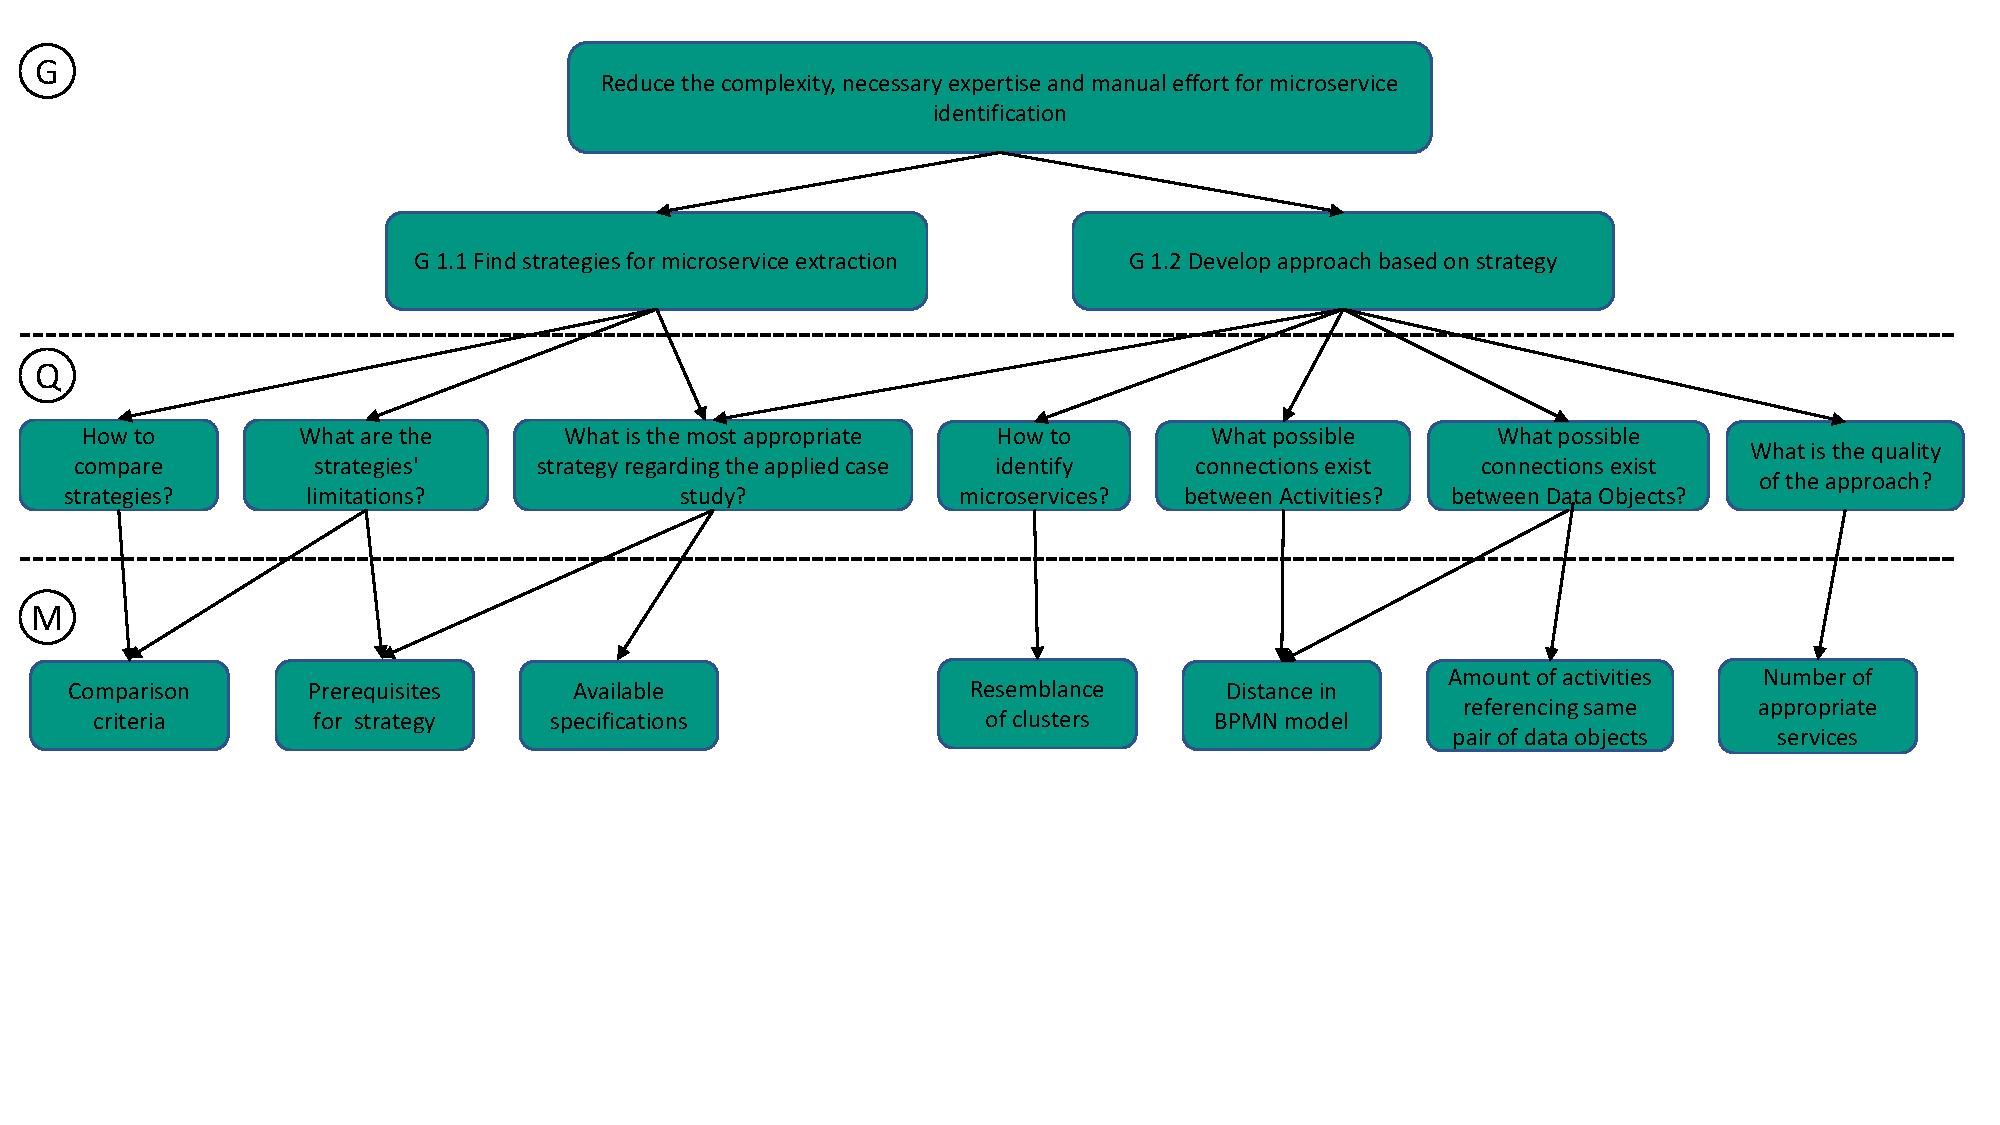
\includegraphics[width=\paperwidth, trim={0 3cm 0 0}]{img/GQM.pdf}
		\caption{GQM Plan}
		\label{fig:GQMPlan}
	\end{figure}
		
		
		
	\end{landscape}
	\clearpage% Flush page
}





